\subsection{Experimento doblaje}
\begin{enumerate}
    \item Al reproducir el archivo de audio original, se logra apreciar la mezcla de dos componentes, una de estas componentes se mantiene constante, se agudiza despeas de un momento, se vuelve a mantener constante en ese tono y  se agudiza nuevamente para mantenerse en constante en ese último tono, es decir, cada vez que se agudizó la señal aumentó su frecuencia; mientras la otra componente se vuelve más aguda, o aumenta su frecuencia,  de forma lineal en tres oportunidades comenzando su incremento en el mismo instante en que la componente constante se agudiza. 
    
    Para el caso en que se reproduce una señal de audio que tiene la mitad del tamaño que tenía el archivo original, en el que se consideran solo muestras pares de dicho archivo, también se pueden distinguir dos componentes, una varía y la otra se mantiene constante tal como en el caso en que se reproduce la señal original. Sobre la componente que varía, se puede notar que esta al principio  aumenta linealmente su frecuencia igual que antes, pero en el segundo y tercer cambio que presenta la componente constante, la que varía posee un incremento lineal hasta que llega un punto en que el la variación corresponde a un  un decremento lineal en frecuencias, apreciándose como un sonido que se agudiza lentamente   y luego se torna cada vez mas grave.
    
    Finalmente, cuando se hace \textit{Downsampling} a la señal original tomando una de cada tres muestras almacenándolas en un vector que tiene un tercio del tamaño del archivo original, nuevamente se distinguen dos componentes, una componente que se mantiene constante presentando ligeros cambios después de unos instantes  igual que en los dos casos anteriores, o suena levemente más agudo, mientras que la otra componente en principio se hace cada vez mas aguda hasta que en un momento comienza a hacerse mas grave, es decir aumenta linealmente su frecuencia y luego decrece también linealmente, al presentarse el primer cambio en la componente constante, la componente que varía presenta un comportamiento similar al antes descrito,  pero esta vez el tiempo que se mantiene el incremento lineal es menor al tiempo  que dura el decrecimiento. Cuando se presenta la última modificación en la componente constante, se aprecia que  la componente que varía comienza aguda y el sonido solo se hace más grave decrementando linealmente su frecuencia.
    
    \item Lo descrito anteriormente, que corresponde a la apreciación auditiva de las señales obtenidas se puede corroborar viendo el espectrograma de las tres señales, la correspondiente al archivo de audio original, la que tiene sólo las muestras pares y la que se obtiene haciendo \textit{Downsampling} con $D = 3$
    
    
    \begin{figure}[H]
        \centering
        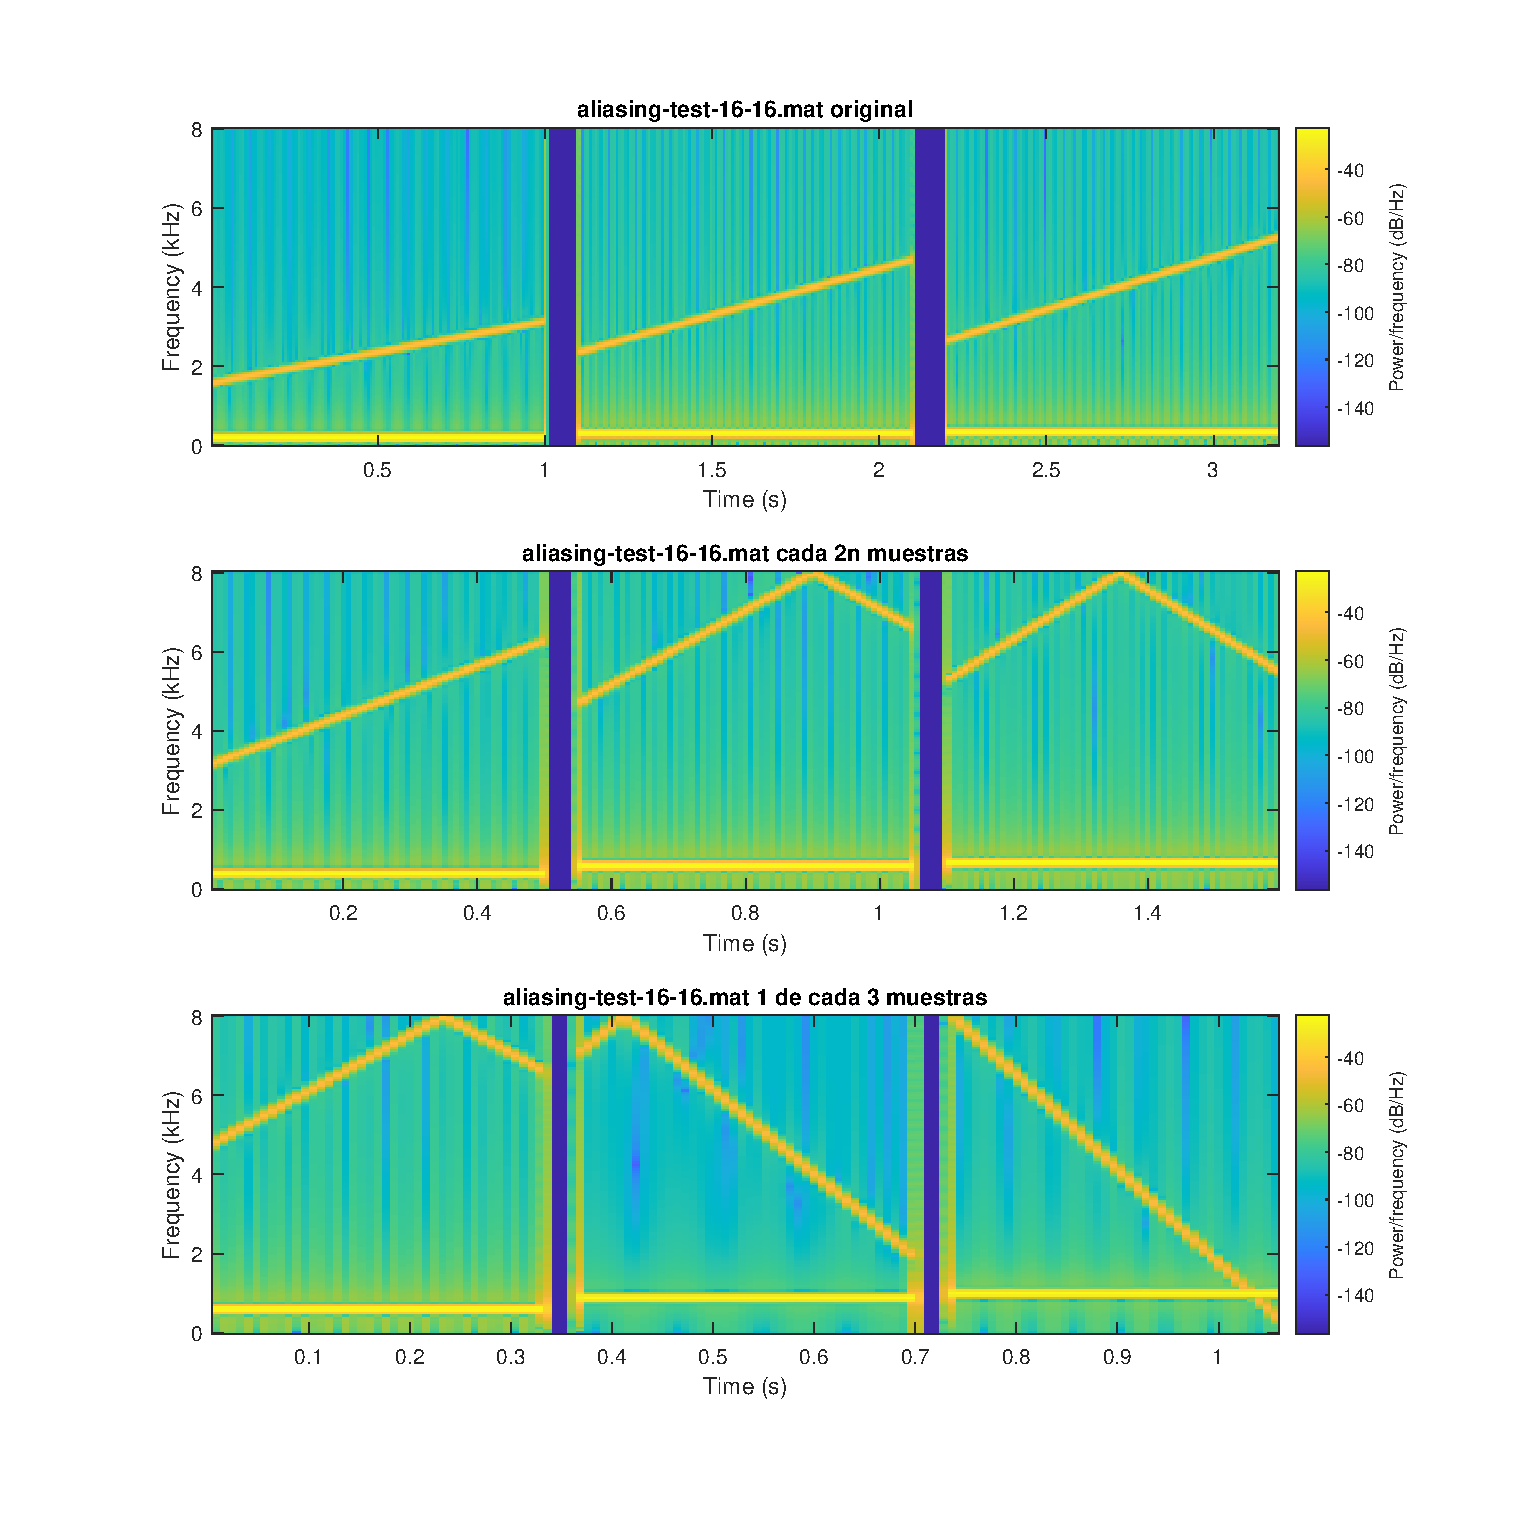
\includegraphics[scale = 0.5]{Imagenes/espectogramas.eps}
        \caption{Espectrograma de las señales obtenidas y reproducidas a partir del archivo de audio \texttt{aliasing-text-16-16}.}
        \label{fig:my_label}
    \end{figure}
    
    
    Observando el  espectrograma correspondiente al archivo de audio original, se puede deducir que la tasa mínima a la que se podría re-muestrear el vector de datos original es de al menos  de los $10.6~kHz$
\end{enumerate}

